\documentclass[10pt,a4paper]{article}
\usepackage[margin=2.2cm]{geometry}
\usepackage{fontspec}
\usepackage{kotex}
\setmainfont{Apple SD Gothic Neo}
\setsansfont{Apple SD Gothic Neo}
\usepackage{amsmath,amssymb}
\usepackage{graphicx}
\usepackage{booktabs}
\usepackage{caption}
\usepackage[dvipsnames]{xcolor}
\usepackage[colorlinks=true,linkcolor=MidnightBlue,citecolor=MidnightBlue,
            urlcolor=MidnightBlue]{hyperref}
\usepackage{titlesec}
\titleformat{\section}{\large\bfseries}{\thesection}{0.6em}{}
\titleformat{\subsection}{\normalsize\bfseries}{\thesubsection}{0.5em}{}
\captionsetup{font=small,labelfont=bf}
\setlength{\parskip}{0.35em}
\setlength{\parindent}{0pt}

\usepackage{mdframed}
\newmdenv[linewidth=0.4pt,linecolor=gray!60,backgroundcolor=gray!5,
          innertopmargin=6pt,innerbottommargin=6pt,skipabove=8pt,skipbelow=8pt]{claimbox}
\newcommand{\claim}[2]{\begin{claimbox}\textbf{주장.} #1\par\smallskip
  \textcolor{gray!70}{\textbf{반증 조건.} #2}\end{claimbox}}

\title{\bfseries 안에서는 세고 밖으로는 안 간다\\[2pt]
\large 그리고 우리가 닫은 문을 다시 열어 보니 열쇠가 없었다}
\author{월드모델 실험실 · 노트 $789 \sim 790$}
\date{2026-08-07}
\begin{document}\maketitle

\section{한 줄}

T$3$(소셜 법칙)에 남은 물음은 하나였다 --- \emph{``도메인을 묶을 수 있나.''}
트랙에 적힌 설계는 \emph{삼분위 곡선 모양으로 군집하고 무리 안 부호 일치를 잰다}
였는데, \textbf{측정을 걸기 전에 읽어 보니 순환이었다} --- 노트 $657$ 이
\textbf{부호가 모양으로 정해진다}는 것을 이미 쟀기 때문이다.

그래서 순환하지 않는 자로 바꿨다: \textbf{A 에서 계단을 배워 B 에 먹이고 B 의
라벨로 채점한다.} 그리고 노트 $657$ 을 재현하려다 \textbf{재현할 수 없다는 것을
알았다} --- 재는 코드가 스크래치패드에 있었고 세션과 함께 사라졌다.

결과는 한 줄로 갈린다. \textbf{감쇠율은 도메인 안에서는 라벨을 잘 설명한다}
(게임 $\rho = +0.49$ · 세계애니 $+0.22$ · 애니 $+0.20$ · 정의 넷 전부).
\textbf{그리고 도메인을 하나도 못 넘는다} --- 교차 순서쌍 $20$개 $\times$ 정의 $4$
에서 \textbf{통과 $\mathbf{0}$}.

\begin{figure}[t]\centering
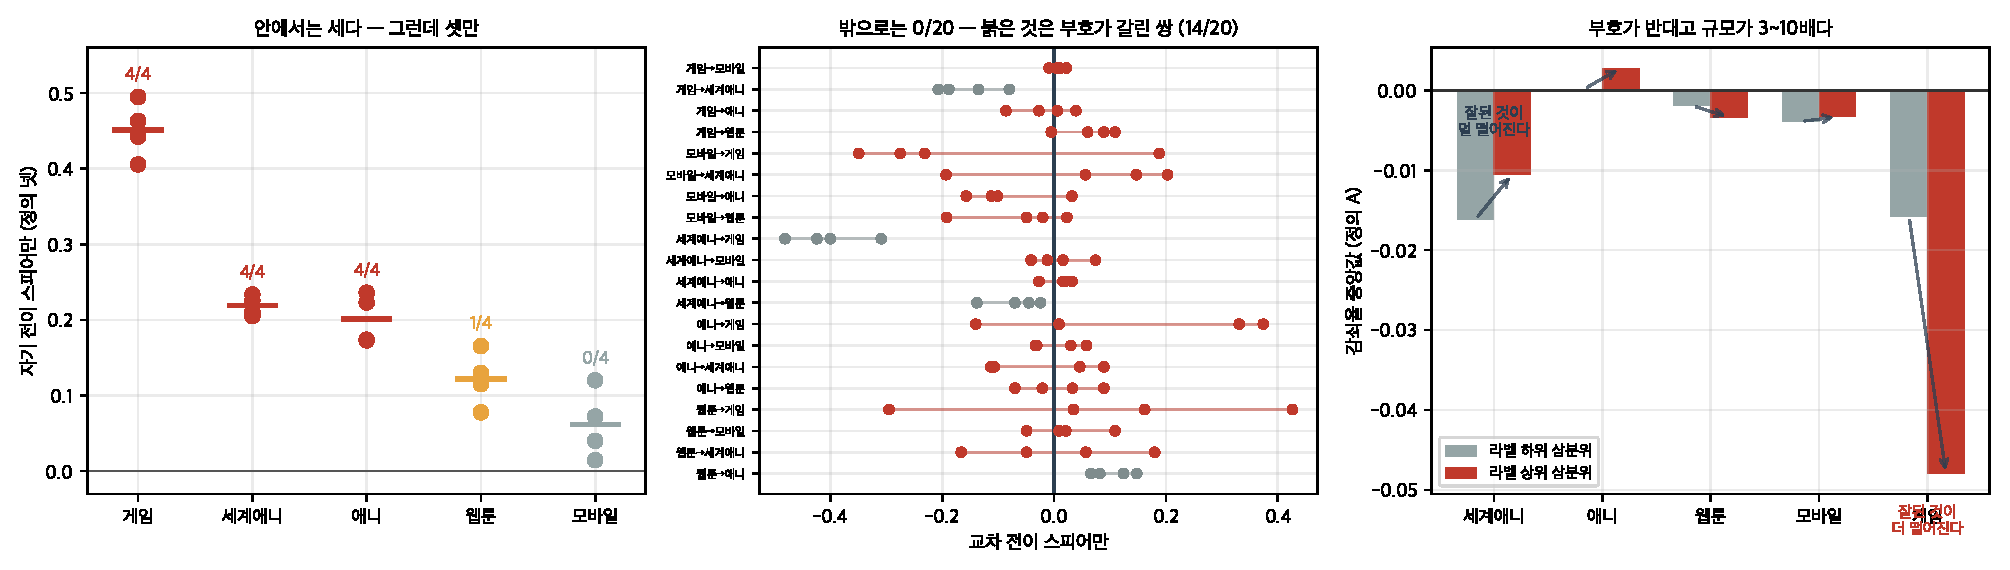
\includegraphics[width=0.99\textwidth]{figs/insideout.pdf}
\caption{왼쪽: \textbf{자기 전이} --- 붉은 것이 정의 넷 전부 통과. 가운데:
\textbf{교차 전이 $20$쌍} --- 붉은 것은 정의에 따라 \textbf{부호가 뒤집히는} 쌍
($14/20$). 오른쪽: \textbf{왜 안 가나} --- 세계애니와 게임은 방향이 반대고 크기가
$3{\sim}10$배 다르다.}
\end{figure}

\section{먼저 --- 우리가 닫은 문을 열어 보니 열쇠가 없었다}

노트 $656 \cdot 657$ 이 이 자료로 T$3$ 의 위키 경로를 닫았다. 그 결론은 대장에
남았는데 \textbf{재는 코드는 남지 않았다.} 대장에는 \emph{``규모 없앤 감쇠율''}
이라고만 적혀 있다.

자연스러운 정의 \textbf{넷을 결과 보기 전에 못박고}(log$45$ · 평균나눔 · log$30$ ·
$7$일비) 노트 $657$ 의 삼분위 무늬를 재현해 봤다.

\begin{center}
\begin{tabular}{lccccc}
\toprule
정의 & 세계애니 & 애니 & 웹툰 & 모바일 & 게임 \\
\midrule
노트 $657$ & 단조 & U & 역U & U & \textbf{U} \\
\midrule
(A) log$45$ & 단조 \checkmark & 단조 & 역U \checkmark & U \checkmark & 단조 \\
(B) 평균나눔 & 단조 \checkmark & U \checkmark & 단조 & U \checkmark & 단조 \\
(C) log$30$ & 단조 \checkmark & 단조 & U & U \checkmark & 단조 \\
(D) $7$일비 & 단조 \checkmark & 단조 & 단조 & U \checkmark & 단조 \\
\bottomrule
\end{tabular}
\end{center}

\textbf{최고가 $3/5$ 다.} 문턱을 $4$ 로 미리 못박아 뒀으므로 그 판정을 하지 않았다.

\claim{\textbf{행 선택이 아니라 정의만 다르다.} 표본 수가 노트 $657$ 과
\textbf{정확히 일치한다}(세계애니 $1{,}128$ · 애니 $396$ · 웹툰 $167$ · 모바일
$150$ · 게임 $149$). 크기는 네 정의 모두 $657$ 의 $1.3{\sim}4.7$배라
\textbf{$657$ 이 더 긴 창을 썼을 가능성이 높다} --- 로그 곡선은 창이 길수록
기울기가 완만하다.}
{그렇다면 다섯째 후보($90$일 창)로 맞출 수 있다. \textbf{지금 추가하지 않았다} ---
결과를 보고 후보를 늘리는 것이 갈래 고르기다. \textbf{새로 사전등록해야 쓴다고
적었다.}}

\subsection*{그래서 규약 $41$ 을 세웠다}

\begin{center}
\textbf{법칙을 재는 코드는 저장소에 둔다.}
\end{center}

노트 $546 \cdot 549$ 는 \emph{``장부와 코드가 따로 자란다''}였고 그때는
\textbf{장부가 앞서 갔다.} \textbf{이번엔 장부만 남고 코드가 없었다.}
\texttt{lab/decay.py} 를 만들고 감사표에 넣었다 --- 이제 사라지면 감사가 잡는다.

\subsection*{그런데 재현 실패가 그냥 실패가 아니었다}

\textbf{정의 넷을 가로질러 무엇이 안정적인지}가 나왔다.

\begin{center}
\textbf{안정}($4/4$): 모바일 U · 세계애니 단조 · \textbf{게임 단조}\\
\textbf{불안정}: 애니(단조·U·단조·단조) · 웹툰(역U·단조·U·단조)
\end{center}

\textbf{노트 $657$ 의 헤드라인이 네 정의 모두에서 안 나온다.} $657$ 은 \emph{``U자가
게임에서 나올 것''}을 예측하고 \emph{``게임 U자 --- 예측이 맞았다''}로 적었다.
\textbf{네 정의 모두 게임을 단조로, 그것도 강하게 낸다}($-0.0158 \to -0.0360 \to
-0.0479$).

\textbf{다만 $657$ 의 결정 규칙 자체는 대체로 산다} --- \emph{``U자 도메인이 둘
이상''}은 A·B·C 에서 각각 $2$개로 통과하고 D 에서만 미달이다. \textbf{``비단조가
있다''는 살고 ``어느 도메인이 U자냐''는 안 산다.}

\section{그리고 정의에 강건한 자로 다시 쟀다}

$657$ 재현을 요구하는 대신 \textbf{더 엄한 자}로 바꿔 새로 사전등록했다 ---
\textbf{네 정의 전부에서 문턱을 넘는 쌍만 통과}($3/4$ 는 통과가 아니다),
\textbf{무리는 양방향}(A$\to$B 와 B$\to$A 가 둘 다 $4/4$).

문턱은 쌍마다 \textbf{B 의 라벨을 $200$번 섞은 순열 영분포의 $2\sigma$} 다 ---
씨앗 SE 가 아니다(노트 $613$).

\begin{center}
\begin{tabular}{lrrl}
\toprule
& 자기 전이 $\rho$(정의 넷) & 통과 & \\
\midrule
\textbf{게임}($149$행) & $+0.41 \sim +0.49$ & $\mathbf{4/4}$ & $z\ 4.8{\sim}6.0$ \\
\textbf{세계애니}($1{,}128$) & $+0.21 \sim +0.23$ & $\mathbf{4/4}$ & $z\ 6.4{\sim}7.6$ \\
\textbf{애니}($396$) & $+0.17 \sim +0.24$ & $\mathbf{4/4}$ & $z\ 3.5{\sim}5.2$ \\
웹툰($167$) & $+0.08 \sim +0.17$ & $1/4$ & \\
\textcolor{BrickRed}{\textbf{모바일}}($150$) & $+0.01 \sim +0.12$ & $\mathbf{0/4}$ & $z\ 0.2{\sim}1.7$ \\
\midrule
\textbf{교차 순서쌍 $20$개} & & \textcolor{BrickRed}{$\mathbf{0/20}$} & $3/4$ 도 $0$ · 양방향 $0$ \\
\bottomrule
\end{tabular}
\end{center}

\textbf{⚠️ 자기 전이는 안에서 맞춘 값이라 부풀려져 있다} --- $5$칸 계단을 같은 행에
채점했고 순열 영분포가 그 부풀림을 안 걷어낸다. \textbf{절대값으로 읽지 말고
도메인 사이 비교로만 읽는다.} 교차 전이는 계단이 남의 도메인에서 오므로 깨끗하다.

\claim{\textbf{노트 $656$ 의 ``부호 일치 $4/8$'' 은 두 물음을 섞은 것이었다} ---
\emph{①} 감쇠율이 그 도메인 안에서 뜻이 있나 \emph{②} 그 함수가 도메인을 넘나.
\textbf{여기서 둘이 갈렸다}: ① 은 세 도메인에서 \textbf{예}($z\ 3.5{\sim}7.6$),
② 는 스무 순서쌍 \textbf{전부 아니오}. \textbf{``부호가 갈린다''가 아니라
``안에서는 세고 밖으로 안 간다''가 맞는 서술이다.}}
{도메인이 \textbf{다섯}이다. $20$쌍이 다 실패해도 여섯째 도메인이 다르게 굴
가능성은 남는다. \textbf{그리고 계단이 $5$칸이라 거친 함수다} --- 더 매끄러운
사상(단조 회귀 · 스플라인)이면 넘어갈 수도 있고, \textbf{안 쟀다.}}

\subsection*{$657$ 이 이상하다고 본 게임이 실은 가장 센 도메인이다}

$657$ 은 게임을 \emph{``U자 · 부호 반대 · 문제 있는 출시가 만든 검색''}으로 읽었다.
\textbf{네 정의 모두 게임을 단조로 내고, 자기 전이가 다섯 중 가장 강하다.}

방향은 \textbf{잘된 게임일수록 더 빨리 떨어진다.} 세계애니는 \textbf{정반대}다.

\claim{\textbf{이것이 ``도메인 상수''의 정체다} --- 잡음이 아니라 \textbf{부호가
반대인 강한 관계 둘}이다. 노트 $656$ 의 부호 $4{:}4$ 는 여기서 나왔다.}
{\texttt{세계애니}$\to$\texttt{게임} 이 네 정의 모두 $-0.31 \sim -0.48$ 인 것은
\textbf{그대로 못 읽는다} --- 게임 $149$행의 \textbf{$58{\sim}61\%$ 가 세계애니
계단의 최하위 칸 하나에 몰린다}(감쇠 규모가 $3{\sim}10$배). 규모 불일치라 예측이
거의 상수이고, 음수는 상위 칸에 떨어진 $25$행이 만든다. \textbf{규모를 도메인 안에서
백분위로 맞추면 달라질 수 있고, 그것도 안 쟀다.}}

\subsection*{그리고 모바일에는 관계가 아예 없다}

모바일 자기 전이가 $\mathbf{0/4}$ 다 --- \textbf{안에서 맞춘 값인데도 자기 순열을 못
넘는다.}

\claim{\textbf{규약 $42$ --- 모양을 읽기 전에 그 관계가 있는지부터 잰다.} 노트
$657$ 이 모바일의 삼분위 U자를 \emph{``비단조 $4/5$''}의 근거로 셌는데,
\textbf{모바일은 감쇠율과 라벨 사이에 관계가 없다.} 관계가 없는 데서 나온 중앙값의
오르내림을 모양으로 읽은 것이다. \textbf{그리고 관계가 없으면 정의를 바꿔도 무늬가
안 바뀐다} --- 모바일만 네 정의 모두 U 였던 것이 그것으로 설명된다.
\textbf{그 안정성을 신호로 읽으면 안 된다.}}
{$150$행이라 검정력이 낮을 뿐일 수 있다. 다만 게임은 \textbf{$149$행으로 $z\ 6.0$}
을 냈으므로 행수 문제로는 설명이 안 된다.}

\section{내 예측이 틀린 방식}

넷 중 셋이 맞았다(교차 $\leq 3$ · 양방향 $0$ · 게임 낀 쌍 안 넘음). 틀린 것은
\emph{``세계애니($1{,}128$행)의 계단이 가장 안정적이라 가장 잘 넘을 것''}이다.

\claim{\textbf{계단의 안정성과 계단의 이식성은 다른 것이다.} 세계애니의 계단은
$1{,}128$행에서 왔고 실제로 안정적이다 --- 그런데 \textbf{게임에서 무너졌다.}
\textbf{상대 도메인의 값 범위가 다르면 안정적인 계단도 못 쓴다.} 이것은 논문 $157$ 의
차원 비용과 같은 자리다 --- \textbf{집안에서 좋은 것이 집 밖에서 좋으리라는 보장이
없고, 그 이유가 매번 다르다}(그때는 열 수, 여기서는 값 범위).}
{범위를 맞추면(도메인 안 백분위로 사상) 넘어갈 수 있다. \textbf{그러면 ``법칙''이
아니라 ``순위 법칙''이고 규약 $27$ 이 경고한 자리다} --- 전 구간 백분위는 편차를
다시 수준으로 되돌린다. \textbf{다음 사전등록의 몫이다.}}

\section{처분}

\textbf{T$3$ 는 쉰다.} 위키 경로는 두 번 닫혔고 \textbf{이번엔 정의에 강건하게}
닫혔다. 자료($2{,}329$건)와 코드(\texttt{lab/decay.py})는 남긴다.

\begin{center}
\textbf{넘기는 것 둘} --- ① \textbf{T$5$} 로: 노트 $790$ 의 부호 반전(게임 대
세계애니)을 \textbf{도메인 임베딩이 담아내나}의 시험 자료로 쓴다. 담아내면
`도메인 상수를 모형이 배운다'는 증거이고, \textbf{못 담아내면 그 아키텍처의
반증이다.} ② \textbf{T$7$} 로: 댓글 시각 API 키 --- (시간 $\times$ 대상) 궤적.
\end{center}

\end{document}
